\subsection{Internal Resistance of the DC Motor $R_m$}
The first parameter to be tested is the internal resistance of the motor $R_m$. This resistance is needed in the motor's transfer function and will be used to determine the other parameters of the motor. 
\subsubsection*{Setup}
\autoref{fig:RmMeasurementSetup} shows a diagram and photo of the measurement set up
\begin{figure}[htbp]
	\centering
	\begin{subfigure}{0.50\textwidth}
		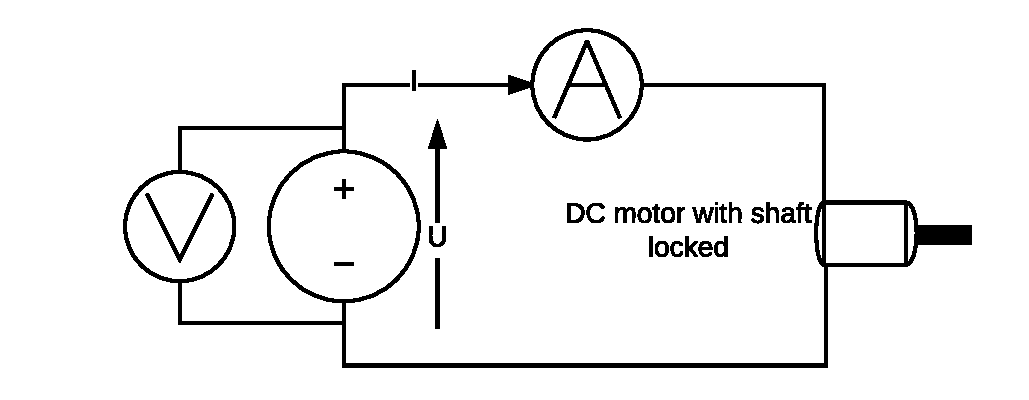
\includegraphics[width=1\textwidth]{figures/appendix/Motor&GearTests/RmTestSetUpDiagram}
		\caption{Diagram of the setup.} \label{fig:LaMeasurementDiagram}
	\end{subfigure}
	\begin{subfigure}{0.40\textwidth}
		\includegraphics[width=1\textwidth]{figures/figureIsComing}
		\caption{Picture of the setup.} \label{fig:LaMeasurementPictures}
	\end{subfigure}
	\caption{The measurement setup.} \label{fig:RmMeasurementSetup}   
\end{figure} 

\subsubsection*{Method}
This test consists of having the motor shaft locked while the voltage is increased by 0.5 V between measurements.

\subsubsection*{Raw data}
\autoref{tab_appendix:RmData} is the plotted evolution of the voltage of the circuit according to the current.

\begin{figure}[htbp]
	\centering
	\caption{Raw data used to determine $R_m$}\label{tab_appendix:RmData}
	\begin{tabularx}{0.35\textwidth}{XX}
		Voltage (V) & Current (A)\\ \toprule \rowcolor{lightGrey}
		0.50 & 0.33 \\
		1.00 & 0.71 \\ \rowcolor{lightGrey}
		1.50 & 1.13 \\
		2.00 & 1.67 \\ \rowcolor{lightGrey}
		2.49 & 2.34 \\
		2.98 & 2.94 \\ \rowcolor{lightGrey}
		3.50 & 3.75 \\
		3.99 & 4.68 \\ \rowcolor{lightGrey}
		4.50 & 5.54 \\
		4.98 & 6.11 \\ \rowcolor{lightGrey}
		5.54 & 6.46 \\
		6.02 & 7.40 \\ \rowcolor{lightGrey}
		6.51 & 8.26 \\
		7.01 & 9.14 
	\end{tabularx}
\end{figure}

\subsubsection{Data Processing}
In order to find the motor's resistance $R_m$, the electrical equations of the motor will be used:
\begin{equation}
	U_m = R_m \cdot i + L_m \frac{di}{dt} + K_e\omega_m
\end{equation}

With the motor shaft locked, $\omega_m = 0$. Moreover, the measurements are made a couple seconds after the change in voltage is made. The current is then constant, canceling its derivative. 

The resulting equation is Ohm's law:
\begin{equation}
U_m = R_m \cdot i
\end{equation}


The measurement of voltage according to the current is presented in \autoref{fig:Rmplot}.
\todo[inline,author=Geoff]{Make lines thicker and titles bigger}
\begin{figure}[htbp]
	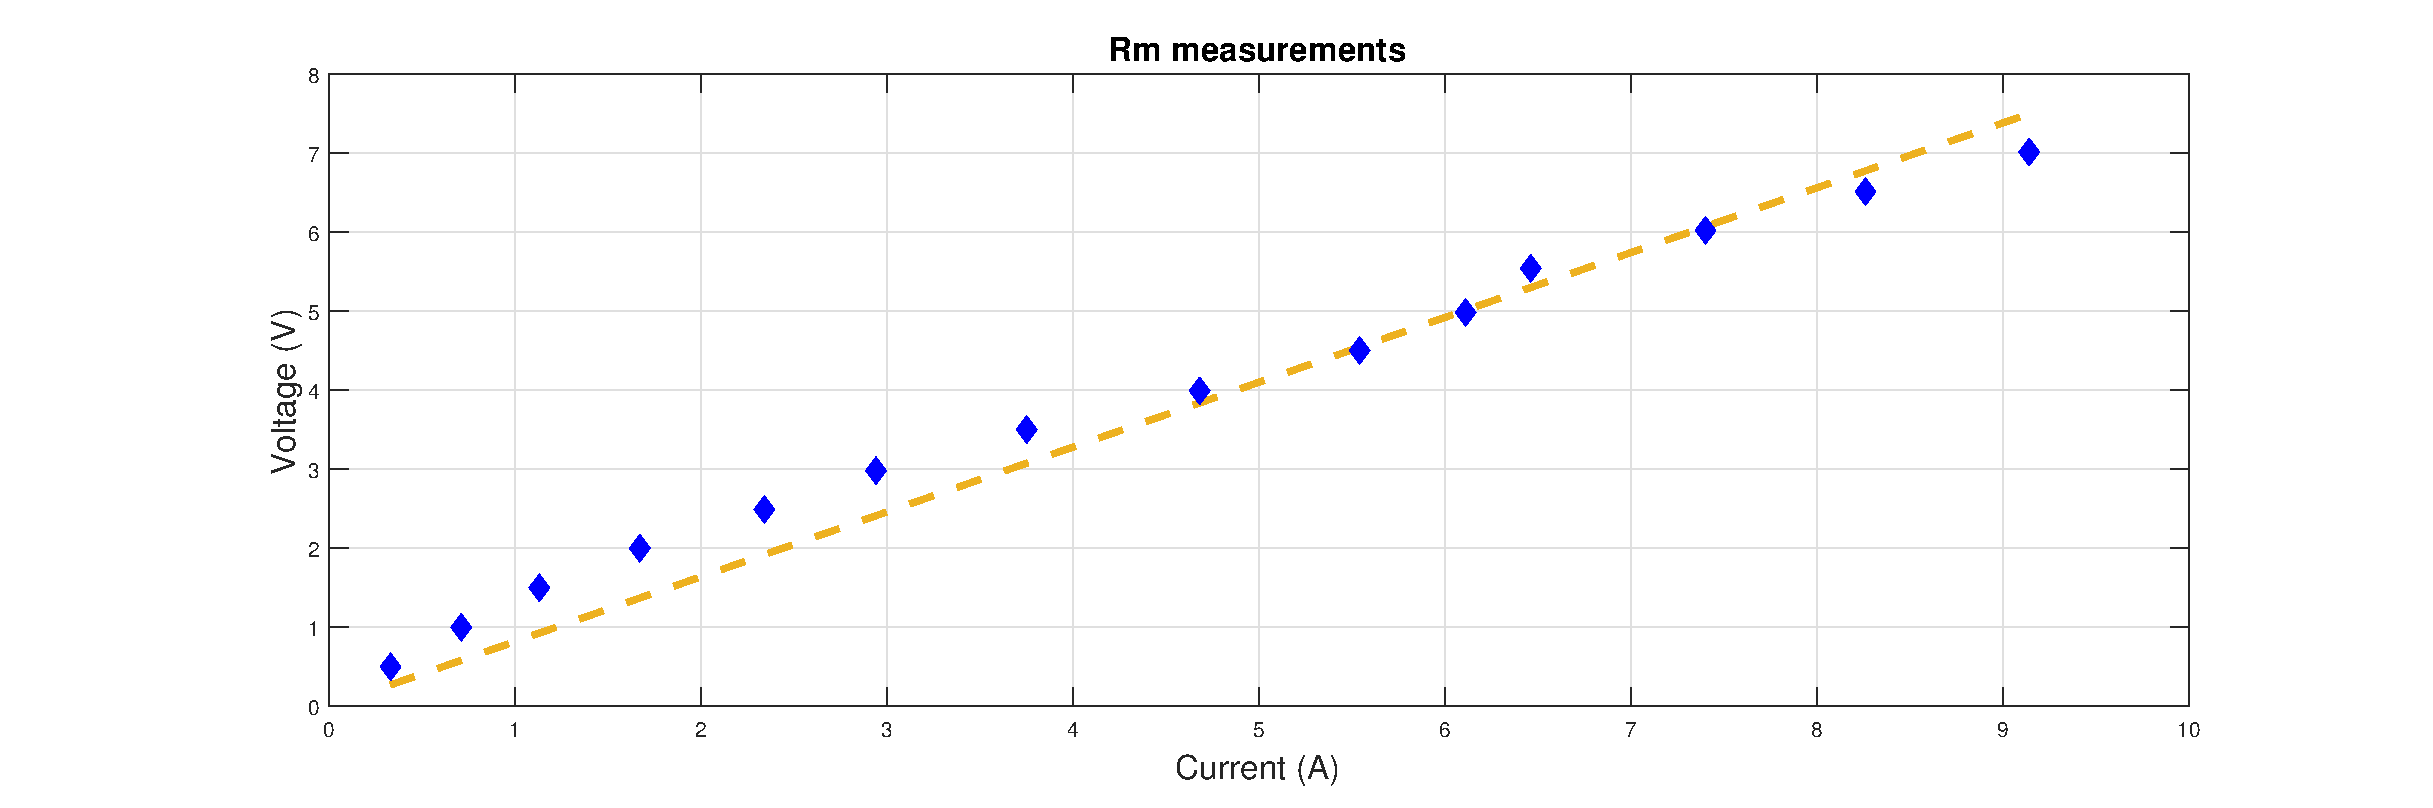
\includegraphics[width=1\textwidth]{figures/appendix/Motor&GearTests/plotRm}
	\caption{Measurement of voltage according to the current} \label{fig:Rmplot}
\end{figure}

$R_m$ is the slope of the linear approximation (in dashed yellow) of the voltage over the current: 
\begin{subequations} \label{eq:LaEq}
	\begin{flalign}
		&U_m = R_m \cdot i \\
		&R_m \approx \SI{0.82}{\ohm}
	\end{flalign}
\end{subequations}


\subsection{Internal Inductance of the DC Motor $L_m$}
\begin{table}[htbp]
	\centering
	\caption{List of measurement equipment and components}\label{tab_appendix:LaSetUp}

	\begin{tabularx}{\textwidth}{lXXXX}
		Name 				& Brand	& Model & AAU-number									\\ \toprule \rowcolor{lightGrey}
		Oscilloscope	& Agilent & 54621D & 33941 	\\
		Powersupply	& Agilent & E3631A & 78577\\ \rowcolor{lightGrey}
		DC motor & Alsthom BBC & F9M2& 08339 
	\end{tabularx}
\end{table}
\subsubsection*{Setup}
\autoref{fig:LaMeasurementSetup} shows a diagram and photo of the measurement set up.
\begin{figure}[htbp]
	\centering
	\begin{subfigure}{0.50\textwidth}
		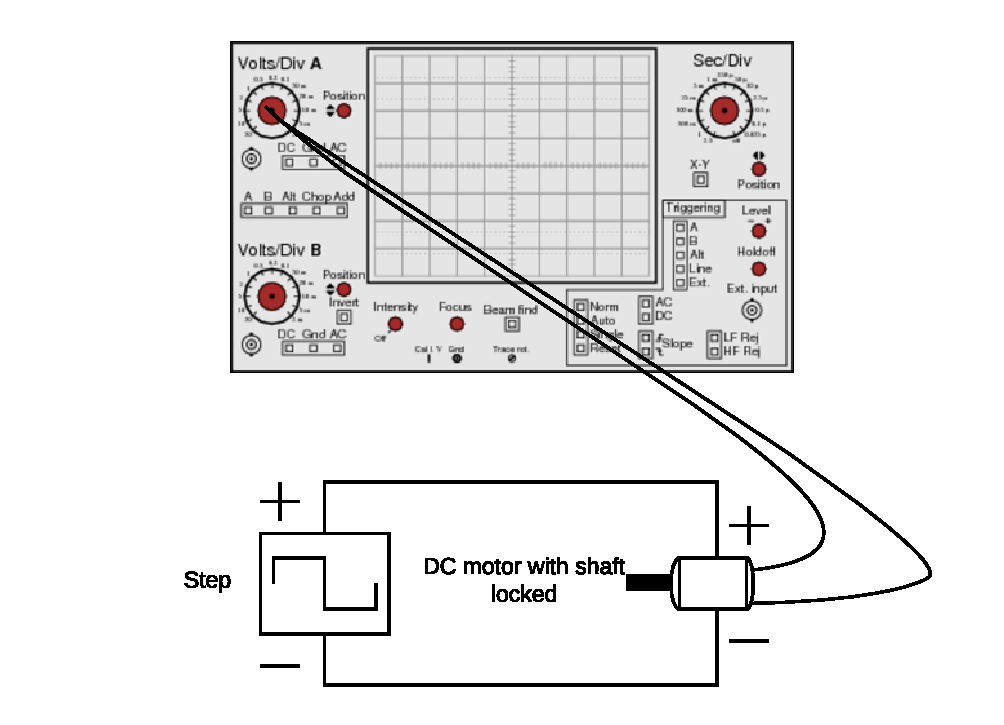
\includegraphics[width=0.7\textwidth]{figures/appendix/Motor&GearTests/LmDiagram}
		\caption{Diagram of the setup.} \label{fig:LaMeasurementDiagram}
	\end{subfigure}
	\begin{subfigure}{0.40\textwidth}
		\includegraphics[width=1\textwidth]{MotorImpedanceTest.jpg}
		\caption{Picture of the setup.} \label{fig:LaMeasurementPictures}
	\end{subfigure}
	\caption{$L_m$ measurement setup.} \label{fig:LaMeasurementSetup}   
\end{figure}

\subsubsection*{Method}
This test consists of having the motor shaft locked while a step is applied. The current is measured through the circuit. With the current step response, the inductance of the motor can be found. 
\subsubsection*{Raw data}
\autoref{fig:LaTestCurrentPlot} is the plotted evolution of the current of the circuit in respect to time.

%\begin{figure}[htbp]
%	\centering
%	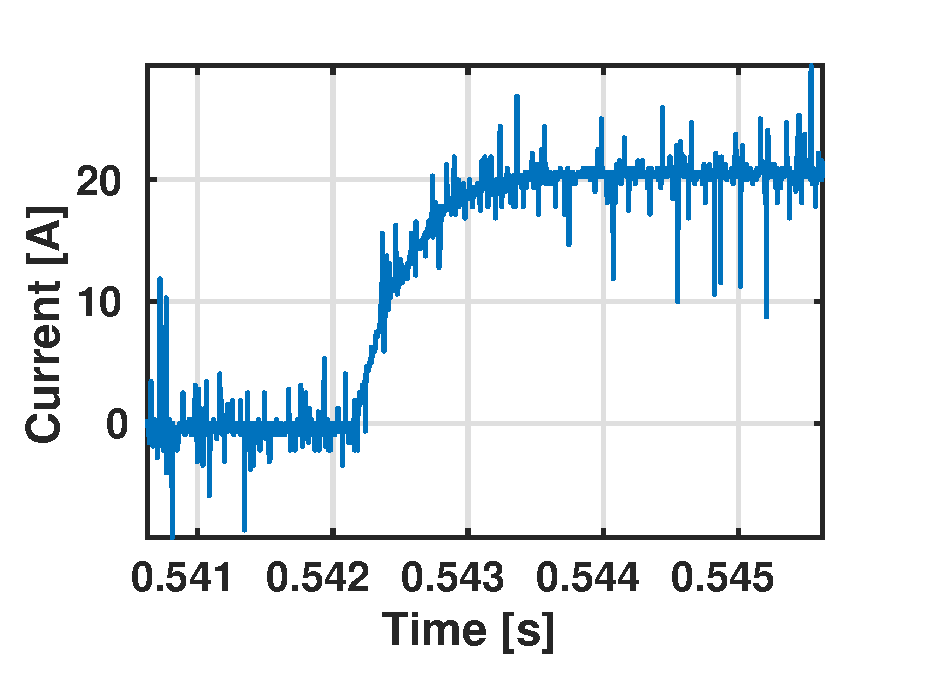
\includegraphics[width=0.7\textwidth]{LaTestCurrentPlot}
%	\caption{Plot of the current in respect to time}\label{fig:LaTestCurrentPlot}
%\end{figure}

\subsubsection*{Data processing}
When the shaft is locked and a step is applied the DC motor's electric equation can be resumed as in \autoref{eq:LaEquation}.
\begin{equation}
	F(s)=\frac{I_a(s)}{U_a(s)}=\frac{\frac{1}{R_a}}{\frac{L_a}{R_a} s+1} \addunit{1}
	\label{eq:LaEquation}
\end{equation}
\startexplain
\explain{$I_a(s)$ is the current in Laplace domain}{1}
\explain{$U_a(s)$ is the body's acceleration}{1}
\explain{$R_a$ is the internal resistance of the motor}{\si{\ohm}}
\explain{$L_a$ is the internal inductance of the motor}{\si{\henry}}
\stopexplain

When a unit step response is applied to the system \autoref{eq:LaEquation} becomes \autoref{eq:LaEquationStep}.

\begin{equation}
F(s)=\frac{\frac{1}{R_a}}{\frac{L_a}{R_a} s+1}\frac{1}{s}=\frac{-\frac{1}{R_a}}{s+\frac{R_a}{L_a}}+\frac{1}{R_a s} \addunit{1}
\label{eq:LaEquationStep}
\end{equation}

\autoref{eq:LaEquationStep} is then put in the continuous time domain to get \autoref{eq:LaEquationStepTime}.

\begin{equation}
f(t)= \frac{1}{R_a} \left(1-e^{-\frac{R_a}{L_a} t}\right) \addunit{1}
\label{eq:LaEquationStepTime}
\end{equation}

\autoref{eq:LaEquationStepTime} means that at $t=\frac{L_a}{R_a}$ the function would give $1-e^{-1}=\SI{63.212055882}{\percent}$ of its settling value. So at \SI{63.212055882}{\percent} of the settling value $t=\frac{L_a}{R_a}$. \\
Since $R_a=\SI{0.82}{\ohm}$ is known, finding $L_m$ becomes trivial.

\subsubsection*{Conclusion}

Since the value of the current at the settling value is \SI{000}{\ampere}. Then \autoref{eq:LaEq} gives the value of $L_m$.

\begin{subequations} \label{eq:LaEq}
	\begin{flalign}
		&\frac{1}{R_a} \left(1-e^{-\frac{R_a}{L_a} \tau}\right)=000 \cdot 0.63212055882 \addunit{\second} \\
		&t = \SI{000}{\second} \\
		&L_a=tR_a \\
		&L_a=\SI{000}{\milli\henry}
	\end{flalign}
\end{subequations}
